\section{根据线性时差校正确定展速度}
\label{sec:5.4}

线性时差校正为求解地震速度的简单图解方法奠定了基础,这种方法对于不是在计算机
内而只是在一张纸上进行的数据分析尤其有用处。此外,这种方法使人们对问题的领悟能远
超出通常计算机化的双曲线扫描所能提供的范围。利用该种方法将会有助于摆脱我们自己关
于测定角度非得从垂直射线开始不可的概念。

最后,这种方法可定义一种速度谱:数据资料观测排列所在之平面经过一种线性可逆变
换之后,就可表示地震速度。

\subsection{测定速度之图解方法}
\label{sec:5.4.1}

设有速度为v之波由位于$(x,z)=(0,z_s)$的点震源出发,在时间t时通过任意点
$(x,z)$,其中
\begin{equation}
v^2t^2=x^2+(z-z_s)^2
\label{eq:ex5.4.1}
\end{equation}
式\ref{eq:ex5.4.1}中的x应以半炮检距h或中心点y代替,这时,t就是双程旅行时间;速度v为岩层
速度的二分之一,而$(z-z_s)$则为距震源之距离。

将式\ref{eq:ex5.4.1}对t微分(保持z为常数),得
\begin{equation}
zv^2t=2x\frac{dx}{dt}
\label{eq:ex5.4.2}
\end{equation}
\begin{equation}
v^2=\frac{x}{t}\frac{dx}{dt}
\label{eq:ex5.4.3}
\end{equation}
图\ref{fig:slnt/tangent}表示,根据式\ref{eq:ex5.4.3}
计算该岩层速度时所需 之三个参量完全可在共中心点道集上测定。

方程\ref{eq:ex5.4.3}可用于估计速度,用以断定地层是
否实际具有恒定的速度。当地层速度属于分层速度$v(z)$
时,很容易证实由方程\ref{eq:ex5.4.3}估计的速度严格等于均方根速度
$v_{RMS}$。首先得注意,切点上到达的一小部分
能量是以恒定的Snell参量出$p=dt/dx$传播经过其全部路
程的。

\begin{figure}[H]
\centering
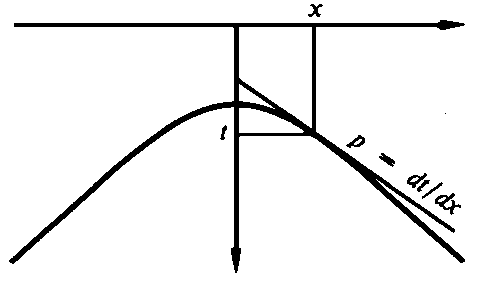
\includegraphics[width=0.65\textwidth]{slnt/tangent}
\caption[tangent]{直线与双曲线时距曲线相切,该直线之斜率p为
任意,因而可取其切点位于信噪比良好之处(据Gonzalez)
}
\label{fig:slnt/tangent}
\end{figure}


要想说明分层介质中的速度,最佳途径就是将它描
述为某种函数$v'(z)$。另一种途径则是挑出某个Snell参
量p并沿具有这个p值的射线开始向下进入地层,当射线
在时刻$t=0$时从地面进入地下时,射线将以速度$v(p,t)$向下移动着。根据$v'(z)$计算
出$v(p,t)$或者由$v(p,t)$计算出$v'(z)$,这属于一种基本性的运算功夫。射线在时间t内旅
行经过的距离x由速度水平分量的时间积分给出,即。
\begin{equation}
x=\int_0^t v(p,t)\sin\theta dt
\label{eq:ex5.4.4}
\end{equation}
以pv代替$\sin\theta$并将常数p提出在积分号外,得
\begin{equation}
x=p\int_0^t[v(p,t)]^2dt
\label{eq:ex5.4.5}
\end{equation}
记住$p=dt/dx$,将\ref{eq:ex5.4.5}代入\ref{eq:ex5.4.3}
\begin{equation}
v_{观测}^2=\frac{x}{t}\frac{dx}{dt}
\label{eq:ex5.4.6}
\end{equation}
则得
\begin{equation}
v_{观测}^2=\frac{1}{t}\int_0^t[v(p,t)]^2dt
\label{eq:ex5.4.7}
\end{equation}
此式证实了下述论断
\begin{equation}
v_{观测}=v_{RMS}
\label{eq:ex5.4.8}
\end{equation}
方程\ref{eq:ex5.4.7}是严格的定义,它无需乎涉及“小炮检距”假设或者“直线射线”假设。

其次让我们来计算层速度。图\ref{fig:slnt/tan2}表示由两个平界面形成的双曲面波至,作两条具有
相同斜率p的直线分别与各该双曲线相切,测定出切点分别为$(x_1,t_1)$和$(x_2,t_2)$。将式
\ref{eq:ex5.4.6}与\ref{eq:ex5.4.4}结合起来,并用下标i表示第i个切点$(x_i,t_i)$,得出
\begin{equation}
x_i\frac{dx}{dt}=\int_0^{t_i}[v(p,t)]^2dt
\label{eq:ex5.4.9}
\end{equation}
假设相继两个同相轴之间的速度为常数$v_{\text{层}}$,于是从具有下标$i+1$
的式\ref{eq:ex5.4.9}中减去具有下标i的式\ref{eq:ex5.4.9},得到
\begin{equation}
(x_{i+1}-x_i)\frac{dx}{dt}=\int_{t_i}^{t_{i+1}}[v(p,t)]^2dt=
(t_{i+1}-t_i)v_{\text{层}}^2
\label{eq:ex5.4.10}
\end{equation}
由此解出层速度$v_{\text{层}}$得
\begin{equation}
v_{\text{层}}^2=\frac{x_{i+1}-x_i}{t_{i+1}-t_i}\frac{dx}{dt}
\label{eq:ex5.4.11}
\end{equation}



\begin{figure}[H]
\centering
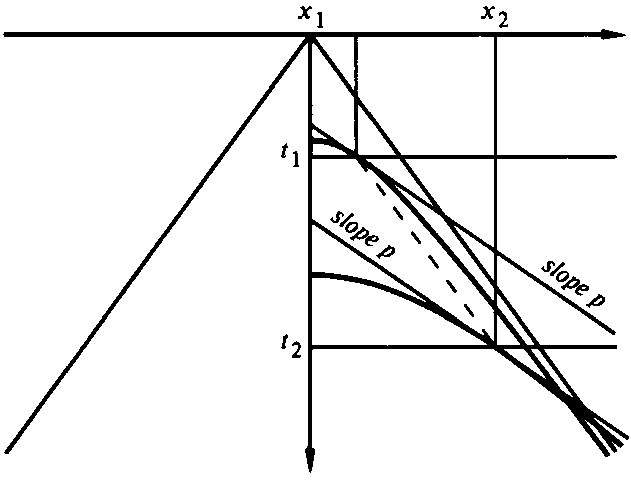
\includegraphics[width=0.65\textwidth]{slnt/tan2}
\caption[tan2]{在共中心点道集上作两条平行直线,使与两个平反射面
形成的反射时距曲线相切(据Gonzalez)
}
\label{fig:slnt/tan2}
\end{figure}

所以,由式\ref{eq:ex5.4.11}可知,利用图\ref{fig:slnt/tan2}中实线直线与虚线直线这两条线的斜率之乘积的
平方根,就可以直接测定出第i反射面与第
$i+1$反射面之间物质的速度。用人工方法在数
据资料上作出两条直线求解层速度的方法优越
于自动速度分析之处在于,你能以图解方式目
估出观测结果对噪音的灵敏度,因而你能在数
据资料中选出最佳炮检距在其上进行观测。

如果你经常性地作这工作,你很快就会发
觉主要工作是要精确作出与各该同相轴相切的
两条直线。当你碰到困难时,你会发现,采用
线性时差校正$t'=t-px$来重新显示数据是有
方便之处的,进行重新显示之后,各直线就不
再是倾斜的而是水平的,这就使得可以使用许
多计时直线中的任何一条直线,现在切点定位
问题变成了一个寻求凸同相轴顶点的问题,这种情形如图\ref{fig:slnt/tan3}所示。

\begin{figure}[H]
\centering
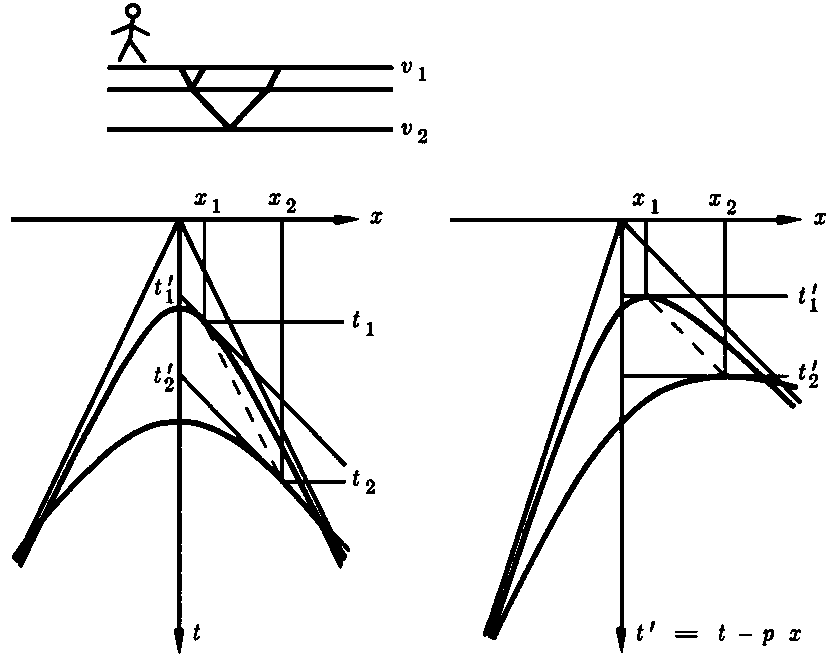
\includegraphics[width=0.65\textwidth]{slnt/tan3}
\caption[tan3]{利用线性时差校正测定层速度(据Gonzalez)
}
\label{fig:slnt/tan3}
\end{figure}

以时间$t'$来表示式\ref{eq:ex5.4.11}则
\begin{equation}
v_{层}^2=\frac{1}{\frac{\Delta t}{\Delta x}}\frac{1}{p}
=\frac{1}{\frac{\Delta t'}{\Delta x}+p}\frac{1}{p}
\label{eq:ex5.4.12}
\end{equation}
在图\ref{fig:slnt/tan3}的右图中测定地层速度,先是测定图中虚线的斜率
即$\Delta t'/\Delta x$,然后把它代入式
\ref{eq:ex5.4.12}内即可。根据用于作图的线性时差校正量大小,已经知道式中的p值。

\subsection{共中心点Snell坐标}
\label{sec:5.4.2}

共中心点倾斜波场分析是一 种比Snell波处理方法更为稳健
的处理地震数据分析的方法,
中心点分析的好处是地层倾角的影响趋向于主要表现在中心点坐标轴上,而地震速度的影响
则主要表现在炮检距坐标轴上。

共中心点分析的缺点在于非物理上可实现。共检波点道集的倾斜叠加模拟的是下行Snell
波,因而你有希望能够写出一个描述该波的微分方程,不管它是多次反射还是横向速度变化,
产生什么结果都没关系。共中心点倾斜叠加则并不模拟物理可实现的任何东西,更不必说存
在有可将这样一种叠加结果进行外推的偏微分方程了,这并不意味着共中心点坐标系统一定
出了什么毛病,但是这点确实使我们更关心Snell波方法了,尽管它在工业界内的应用完全
不是突飞猛进地増长。

值得密切注意的是某些人进行共中心点倾斜叠加比共检波点倾斜叠加还容易,这是因为
在共中心点上,双曲面顶点必然是位于零炮检距上,Fresnel带的位置可以很容易预测出来,
因而内插和丢失数据问题就大大得到缓和。

地震数据是在时间、检波点、炮点和深度坐标系统$(t,g,s,z)$内采集的。现在要定
义一种新的四分量系统,中心点按通常的方式定义
\begin{equation}
y(t,g,s,z)=\frac{g+s}{2}
\label{eq:5.4.13}
\end{equation}
旅行时间深度利用钻井内的垂直相速度$v/\cos\theta$来定义,为尽可能地方便,采用双程旅行时
间$\tau$\footnote{
$\theta$是射线与垂直坐标轴z之间所夹角度。---译者
}。
\begin{equation}
\tau(t,g,s,z)=2z\frac{\cos\theta}{v}
\label{eq:5.4.14}
\end{equation} 
其次定义地面炮检距$h'$,我们将不采用炮检距的老定义。在这种新定义方法情形下,炮点与
检波器不是直接向下移而是沿射线向下移,如$h'$是按下列关系定义的,就可以如此
\begin{equation}
h'(t,g,s,z)=\frac{g-s}{2}+z\tau\theta
\label{eq:ex5.4.15}
\end{equation}
由$h'$的这种新定义可知,在$h'$为常数的情形下,炮点与检波点之间距$(g-s)$将随深度z之
増大而减小。

从点震源观测排列之旅行时间$t$减去相应的线性时差,现将它定义为线性时差校正时间、
或简写为LMO时间(linear moveout
time),因此,在任何深度z时的$LMO$时间等于$t-p
(g-s)$。由于已将h'定义为地表半炮检距,故将t'义为地表LMO时间。根据已延拓至深
度z之排列的LMO时间,再加上该排列的旅行时间深度$\tau$,可把地面上的LMO时间$t'$定义为
\begin{equation}
t'=t-p(g-s)+\tau
\label{eq:5.4.16}
\end{equation}
你也许喜欢将式\ref{eq:5.4.16}
想像成是“斜着”的上行波时间延迟,比如把它看成$t'=t_{lMO}+(z_{slant}/v)$,
不论那种情形,形式上都是
\begin{equation}
t'(t,g,s,z)=t-p(g-s)+2z\frac{\cos\theta}{v}
\label{eq:5.4.17}
\end{equation}

% 海水层底部散射往往很强,使得很难采用常规处理方法压制它。在\ref{sec:3.2}节中,我们已了
% 解其原因在于点溫散射意味着有双曲线型波至,它具有陡倾角,其到达时间一般比水层底部
% 反射时间要晚,因而会误认为它们具有沉积地层的叠加速度而不是水层速度。这时所需要的
% 是作两种倾角滤波,一种是抑制以非垂直角度离开各炮点的波,另一种则是抑制以非垂直角
% 度到达各检波点的波。现今的野外组合其滤波作用系以空间频率$k_x$为基础,如记录设备采用倾
% 角$(k/\omega)$的滤波而不是采用空间频率的滤波,资料中将会留有更多高频能量。\ref{sec:2.5}节中所
% 述具有时间因果性的递归倾角滤波在这里可能会起很好的作用。


% \subsection{Snell波的合成}
% \label{sec:5.3.3}

% 设我们用野外数据人工合成了一个下行的Snell波,然后设想一下上行波将会显得如何,
% 以及它将如何把有关地下界面的信息带给我们。

% 进行倾斜叠加要取测线上的数据$P(s,g,t)$,它是炮点位置s、检波器位置g和旅行时
% 间t的一个函数。然后,要在炮点遍及的范围内求和,从而合成作出犹如应当是由下行Snell波
% 发生了反射才能被记录到的上行波$U(g,t)$。即使可能存在有速度横向变化和多次反射,
% 情形仍应如此,不受影响。

% 因为涉及到三种不同类型的时间,求和过程有点混乱:
% t=点震源野外记录内的时间。\\
% $t'=t-p(g-s)$=解释时间。仅在$t'=0$之后才看得见最浅的反射面。\\
% $t_{pseudo}$=具有移动震源之Snell假想排列记录内的时间。\\

% 在水平成层地层情形下,假想排列记录内的时间$t_{pseudo}$具有特定的特征:你将检波点坐标
% 移出越远,回声反射就会到达越晚。根据下列关系可从野外排列记录的时间t直接变换为解释时间t':
% \begin{equation}
% t'=t_{pseudo}-px=t-p(g-s)
% \label{eq:ex5.3.1}
% \end{equation}
% 图\ref{fig:slnt/snellwave}示意绘出了下行Snell波的情形。

% \begin{figure}[H]
% \centering
% 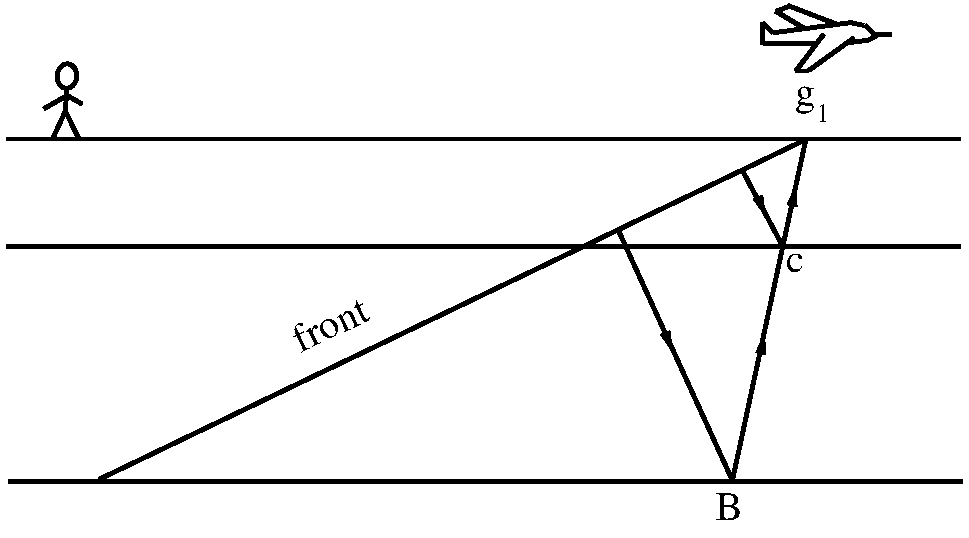
\includegraphics[width=0.65\textwidth]{slnt/snellwave}
% \caption[snellwave]{Snell波的波阵面由两个地层反射,携带信息
% 上行返回至检波器$g_1$
% }
% \label{fig:slnt/snellwave}
% \end{figure}

% 图\ref{fig:slnt/cspss}所示是一种假设的共检
% 波点道集,将该道集求和可模拟出图
% \ref{fig:slnt/snellwave}中所见到的位于$g_1$上之Snell波。在图\ref{fig:slnt/snellwave}
% 中的由C点至B点的横向偏离距离与图\ref{fig:slnt/cspss}中相应的距离(图\ref{fig:slnt/cspss}中的两
% 个位置上)是完全相等的。对所有的检波点
% 重复进行上述沿炮点坐标的求和过程,即可由下行Snell波作出合成上行波。

% \begin{figure}[H]
% \centering
% 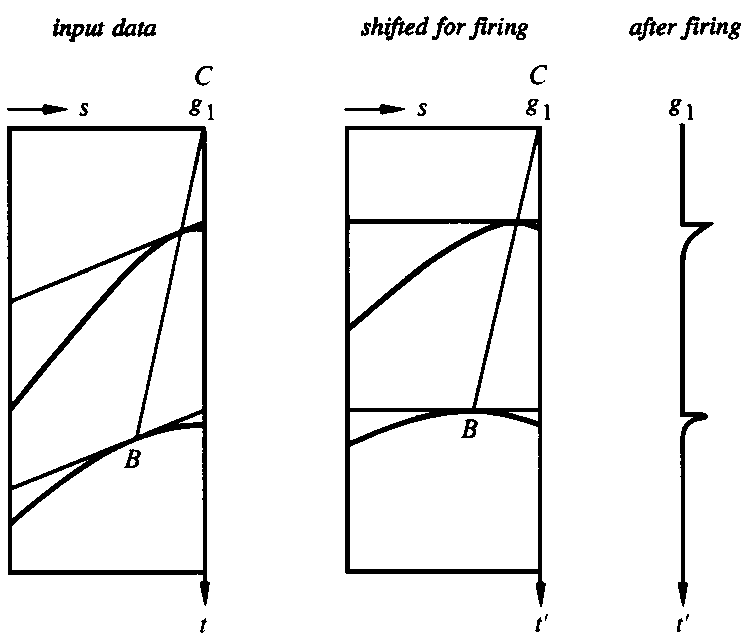
\includegraphics[width=0.65\textwidth]{slnt/cspss}
% \caption[cspss]{左图是两个平反射界面情形下的位于
% 检波点$g_1$上的共检波点道集。中图表示,为准备用遍及炮点
% 坐标s进行求和而产生合成Snell波,数据已根据线性时差校正作
% 了时移。右图所示是检波点$g_1$上所记录到的Snell波记录道。
% Snell波的地震剖面由许多像$g_1$的记录道并列组成。
% }
% \label{fig:slnt/cspss}
% \end{figure}

% 因为仅在$t'=0$之后才看见找层反射面,而且水平地层的回声反射不同于
% 假想的Snell波,其到达并不具有水平方向
% 时差,所以可将变量$t'$称作是解释坐标。在水平地层情形下,对横向位置进行检测
% 得依靠反射系数的横向变化。在图\ref{fig:slnt/snellwave}
% 中,关于B点的反射强度之信息是在右侧
% 的$g_1$点上记录到的,不是像常规叠加那样在B点的正上方之处才能见到它。为了得到完美解
% 释结果,因而得额外要求把所接收数据移动到一个适当的横向位置上去。

% 图\ref{fig:slnt/interpcoord}所示是与图\ref{fig:slnt/snellwave}和\ref{fig:slnt/cspss}相同之两个平界面,但在A、B和C各点上还有异常的反射系数,A点位于B点正上方,
% 由B点所反射的波其路程直接通
% 过C点,再从C点到达检波点$g_1$。 
% 相继各个画面所示均为与这三个
% 点有关的绕射双曲线。注意,从
% 两个平界面发生反射的假想
% Snell波其时差变化率均为办由 
% 散射点B与C形成的双曲线
% 与各该Snell波分别在a、b与c各 
% 点上相切;注意b与c位于仍点正
% 下方的情形,是因为它们全都沿 
% Snell参量为p的一个射线路程排
% 列成行而形成的。由于不论入射 
% 波场情形如何,最早到达的波至
% 必然应位于散射点之正上方,所 
% 以右上图中的A、B和C各点均应
% 位于各该双曲线的顶部。转换为 
% 左下图中的解释坐标t'时,能得
% 到的主要好处是来自水平地层的 
% 波至都变成水平的了。但是要注
% 意,各该双曲面业已变得偏斜。
% 当把我们的注意力局限于具有微
% 小时差的那一部分波至时,我们
% 可以发现关于异常反射系数的信
% 息全部都位于a、b和c各点邻域
% 内,而这些点原来都是处于双曲线的侧翼上的。不把相应数据向左侧横向移动,比方说,
% 移至$g'=g-f(t')$,这些点是不会占有正确几何位置的,亦即不会占据原有的A、B和C点的
% 位置;作过横向移动后,a点将位于b点之上。正确的移动量大小$f(t')$是一个涉及到速度分析
% 的问题,从属这种问题的速度分析将在下节讨论。

% \begin{figure}[H]
% \centering
% 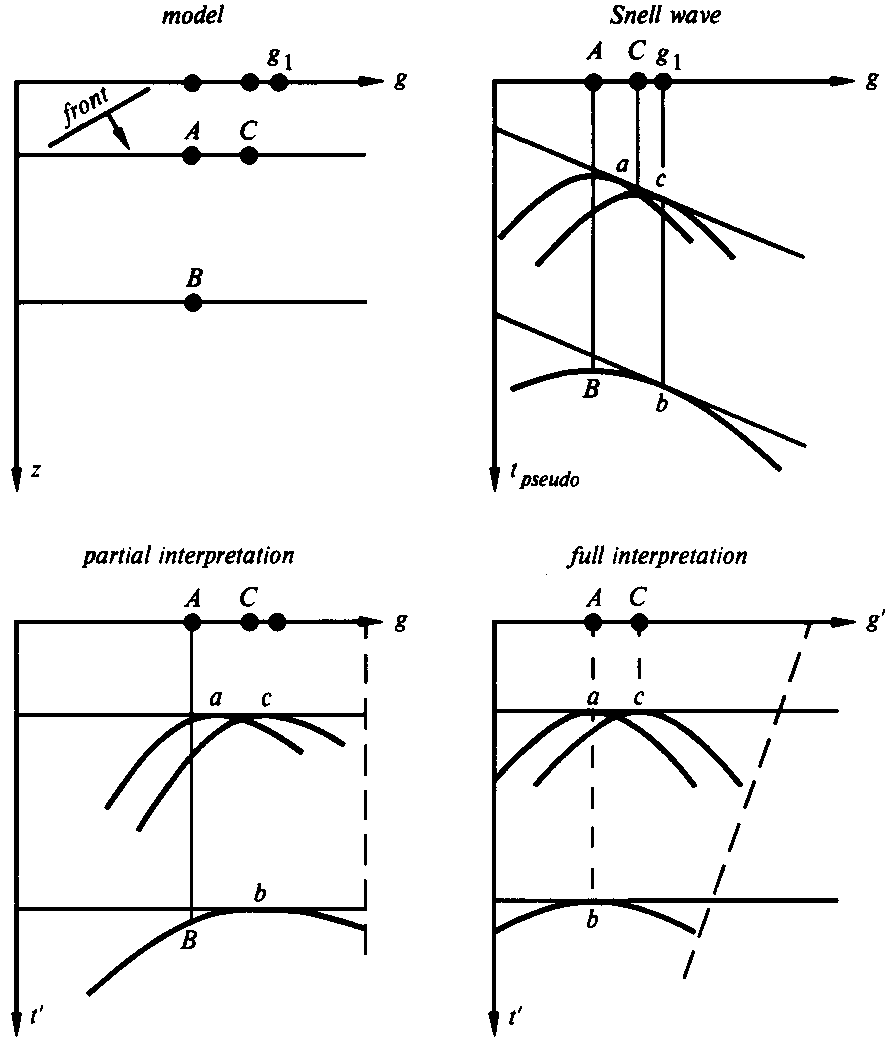
\includegraphics[width=0.65\textwidth]{slnt/interpcoord}
% \caption[interpcoord]{左上图为两个反射面上的三个点散射体义A,B,C。右上图
% 为所期望之Snell波。左下图为经过线性时差校正之后的Snell波。
% 右下图为转换至完整的解释坐标之后的情形,在最后的这个结果
% 中a,b与c各点均已位于幵始时的A、B与C各点位置上了
% }
% \label{fig:slnt/interpcoord}
% \end{figure}

% \subsection{Snell波出了啥毛病?}
% \label{sec:5.3.4}

% 在建立平方根方程以前,我曾经认为进行地震数据分析的唯一正确途径就是把它分解成
% Snell波。既然一个Fresnel带看来不过就大约10°左右,要不了多少Snell波也就行了。只需
% 少量剖面曾经是很重要的。因为七十年代的计算机能力很有限。当时我知道藉助于一个平方
% 根方程每个Snell波都是可分析的,而且知道即使是多次反射也可以采用《地球物理数据处
% 理基础》一书中和本书\ref{sec:5.6}节中所述方法来加以处理。从理论上说,这种办法可算得上是对完
% 全难以分析的CDP叠加所作过的一项重大改进了
% 。然而,对于下行Snell波来说,存在有一个
% 实际问题,这就是:当它们离开地表面之后不久就遇到横向速度不均匀性,它们也许早就
% 变得很复杂了。虽然我对它们将会有什么最终作用还不能肯定,我是不再相信Snell波是一
% 种包治百病的灵丹妙药了。但是,许多波都表现出它们有一点儿像是Snell波,这一点触动
% 了我要去建立发展一种对Snell波来说是理想的坐标系统,而对有一点像是Snell波的那些波
% 来说则是有效的坐标系统。

% \subsection{横向不变性}
% \label{sec:5.3.5}

% 垂直入射力$p=0$平面波震源在水平层状介质内产生的反射波场具有横向不变性,换言
% 之,有关波场的观测与理论在这种情形下所具有的形式均属$P(t)\times const(x)$。在任何特定的
% 非零值情形下的Snell波也都是横向不变的,就是说,利用新坐标
% \begin{subequations}
% \begin{equation}
% t'=t-px
% \label{eq:ex5.3.2a}
% \end{equation}
% \begin{equation}
% x'=x
% \label{eq:ex5.3.2b}
% \end{equation}
% \label{eq:ex5.3.2}
% \end{subequations}
% 则横向不变性可由下述陈述给出
% \begin{equation}
% P(x,t)=P'(t')\times const(x')
% \label{eq:ex5.3.3}
% \end{equation}
% 显然,当一个貌似二维的问题可以简化成一维问题时,会产生重大概念上的好处,更不用说
% 采样和计算上的好处了。在继续进行讨论之前,要研究一下方程\ref{eq:ex5.3.3}直到你确实理解
% 了当如条件\ref{eq:ex5.3.2b}所述$x'=x$时,为什么波场可以随x而变化但却是x'的一种常值函数。


% 坐标系统\ref{eq:ex5.3.2}是延迟坐标系统,不是一种运动坐标系统。在固体地球物理学中,
% 采用运动坐标系统进行计算是很糟糕的,地层内的速度函数从来不是时变的(time-variable),可是在运动坐标系统内它却成为时变的了,这会增加计算的复杂性。我们的目标是采用
% 某一模型速度由数据形成影像,该速度是所有空间维次的一项函数。但是所利用的坐标系统
% 将具有这么一种参考速度,它仅仅是深度之函数。

% \subsection{Snell波的坐标系统}
% \label{sec:5.3.6}

% Snell波有三个固有平面,受此启发,可用它们构成一坐标系统,第一个平面是恒定深
% 度z处的地层平面,其中包括地表面。第二个是射线平面。第三个是运动着的波阵面平面,
% 当速度随深度而变化时,该平面变成曲面。

% 下列方程定义了Snell波坐标系统
% \begin{subequations}
% \begin{equation}
% z'(z,x,t)=z\frac{\cos\theta}{v}
% \label{eq:ex5.3.4a}
% \end{equation}
% \begin{equation}
% x'(z,x,t)=z\tan\theta+x
% \label{eq:ex5.3.4b}
% \end{equation}
% \begin{equation}
% t'(z,x,t)=z\frac{\cos\theta}{v}-x\frac{\sin\theta}{v}+t
% \label{eq:ex5.3.4c}
% \end{equation}
% \label{eq:ex5.3.4}
% \end{subequations}

% 方程\ref{eq:ex5.3.4a}利用钻孔中见到的垂直相速度直接定义了旅行时间深度,地层内部的分
% 界面都正好是恒定z'值处的平面。

% 令方程\ref{eq:ex5.3.4b}所定义的x'等于常数,比如说,等于$x_0$,则得出射线方程,即
% $(x-x_0)/z=-\tan\theta$,不同的$x_0$值代表不同的射线。

% 令方程\ref{eq:ex5.3.4c}所定义的t'等于常数,则给出运动着的波阵面之方程。要看出这点
% 令$t'=t_0$并注意在恒定x值时,你看到的是钻井中的速度,而在恒定z值时,你看到的是飞机
% 的速度。

% 从数学上说,具有三个未知数的一个方程定义了一个平面,所以,令式\ref{eq:ex5.3.4}中任
% 何一个方程的左端为常数,就得出在空间内定义了一个平面的方程。为进行实际检验,
% 不妨考虑一下两个平面相交的情形。使波阵面停留不动得要求$dt'=0$,利用方程\ref{eq:ex5.3.4c},得出
% \begin{equation}
% dt'=0=\frac{\cos\theta}{v}dz-\frac{\sin\theta}{v}dx+dt
% \label{eq:ex5.3.5}
% \end{equation}
% 将该恒定波阵面方程$dt'=0$同恒定深度方程$dz'=dz=0$结合起来,得出了熟悉的关系式
% \begin{equation}
% \frac{dt}{dx}=p
% \label{eq:ex5.3.6}
% \end{equation}

% 在坐标平面是非正交平面时,就说该坐标系统是仿射坐标系统(affine coordinate
% system)。利用像\ref{eq:ex5.3.4}那样的仿射坐标,我们无疑易于控制计算,但是我们往往确实也得
% 遇上给我们自己造成混乱的问题,例如,当我们显示海上野外资料的活动画面时,我们看到
% 的是一系列共炮点道集$(h,t)$平面;相继的平面就是相继的炮点,所以当我们打算在正交
% 坐标$(y,h)$或$(s,g)$中考虑问题时\footnote{
% y为中心点坐标,h为半炮检鉅,g为检波点坐标,s为炮点坐标。 ---译者
% },数据是显示在$(s,h)$平面中的。采用仿射坐
% 标时,我发现最容易忘掉坐标轴而考虑用垂直的平面来代替。炮点坐标轴s可以被当作是一
% 个共检波点平面来考虑,比如说,当作是$cg$。所以,我把海上勘探数据活动电影当作是存在于
% $(cs,ch,ct)$空间中。在这个活动电影中,另一个平面,实际上是一个平面族、即共中心
% 点平面cy,随同数据的“分层结构”(见\ref{sec:3.0}节)而一起扫描通过屏幕。

% 要在速度随深度而变化时定义Snell坐标,仅需要仔细地解释方程\ref{eq:ex5.3.4}。首先,所有
% 的角度必须利用Snell置换$Sin\theta=pv(z)$通过p来表示,然后z必须赴处用对z的积分来代替。


% \subsection{Fourier空间中的Snell波}
% \label{sec:5.3.7}

% 根据偏微分方程连锁法(chain rule),应有
% \begin{equation}
% \begin{pmatrix}
% \partial_t \\
% \partial_x \\
% \partial_z 
% \end{pmatrix}
% =\begin{pmatrix}
% t_t' & x_t' & z_t'\\
% t_x' & x_x' & z_x'\\
% t_z' & x_z' & z_z'
% \end{pmatrix}
% =
% \begin{pmatrix}
% \partial_{t'} \\
% \partial_{x'} \\
% \partial_{z'} 
% \end{pmatrix}
% \label{eq:ex5.3.7}
% \end{equation}

% 在Fourier空间内,上述方程中涉及时间t与水平坐标x的部分可解释为
% \begin{subequations}
% \begin{equation}
% -i\omega=-i\omega'
% \label{eq:ex5.3.8a}
% \end{equation}
% \begin{equation}
% ik_x=+p\omega'+ik_x'
% \label{eq:ex5.3.8b}
% \end{equation}
% \label{eq:ex5.3.8}
% \end{subequations}
% 在线性时差校正(对x'保持恒定)之后变得平缓的同相轴能量具有特殊意义,对于这类能量应
% 有$\partial/\partial x'=ik_x'=0$,于是将式\ref{eq:ex5.3.8a}与
% \ref{eq:ex5.3.8b}结合起来可得出熟悉的关系方程
% \begin{equation}
% p=\frac{k}{\omega}
% \label{eq:ex5.3.9}
% \end{equation}

% \subsection{习题}
% \label{sec:5.3.8}
% \begin{enumerate}
% \item 试解释图\ref{fig:slnt/cspss}中的s坐标轴应如何选取符号。
% \item 方程\ref{eq:ex5.3.4}属于上行Snell波的情形,试问:适用于下行Sneir波的将是何种坐
% 标系统。
% \item 试在坐标系统\ref{eq:ex5.3.4}内表示标量波动方程。忽略其一阶导数项。
% \item 试按照Fourier变量$(\omega ',k_z',k_x')$来表7K标量波动方程的波散关系。
% \end{enumerate}












